\documentclass[10pt,a4paper]{article}
\usepackage[utf8]{inputenc}
\usepackage{amsmath}
\usepackage{amsfonts}
\usepackage{float}
\usepackage{amssymb}
\usepackage{graphicx}
\usepackage{url}

\author{Yasar Mahomed Abbas, Franziska Pannach, \\Danielle Russell, Yuvika Singh}
\title{Report Ontologies and Knowledge Bases}

\begin{document}
\maketitle


\section{Objective and Motivation}
Folk and Fairy tales are a substantial part of oral history. They play an important role in the cultural heritage of regions, nations or cultural minorities. In European context, fairy tales have been collected and editored by the Grimm brother's in the beginning of the 19th century.\cite{Grimm1857} In the African context, the oral tradition of folk tales existed way longer. Presumably, African folk tales are therefore different than European fairy tales in terms of structure and motifs. 
This project aims to construct an ontology of African folk tales following the approach of Russian folklorist Vladimir Propp. We hope to not only collect and structure African folk tales, but also investigate how they follow Propp's formalism and how motifs and agents are verbalised.
Hence, the ontology is going to contain: 

\begin{itemize}
	\item The Proppian functions and entities encoded within. 
	\item Specific folk tale motifs according to the Aarne-Thompson-Uther Index (ATU). 
	\item The representation of the functions and motifs in selected African Folktales. 
\end{itemize}


\section{Domain}
	\subsection{Motifs Indexes}
	Folk tales motifs are usually classified by two motif indices. The Aarne-Thompson-Uther index (ATU)\footnote{\url{http://www.mftd.org/}} is used to classify tales into one category. The categories are relatively wide, describing the main story line of the tale. Therefore, each tale can only have one ATU type. In contrast, the Thompson-Motif-Index (TMI) is more fine grained, describing single motifs, i.e. repeated elements, e.g. characters. The TMI motifs are organized in a hierarchical structure. A tale can be described with more than one TMI motif.\footnote{\url{https://sites.ualberta.ca/urban/Projects/English/Motif_Index.htm}}    
	\subsection{Propp Functions} 
	Russian folklorist Vladimir Propp introduced 31 invariant functions describing the morphology of the Russian magic folk tale. In his ground breaking 1928 work 'Morphology of the Folk tale', he argues that the narrative of folk tales always follows the same pattern. The narrative functions and the \textit{Dramatis Personae} (agents in the story) he introduced are strictly defined and specify recurrent units from which the tales are constructed. 
	Propp \cite{propp1968} set four axioms: 
	
	\begin{enumerate}
	
		\item Functions of characters serve as stable, constant elements in a tale, independent of how and by whom they are fulfilled. They constitute the fundamental components of a tale.
		\item The number of functions known to the fairy tale is limited.
		\item The sequence of functions is always identical.
		\item All fairy tales are of one type in regard to their structure.   
	
	\end{enumerate}
	
The high formality of this structuralism allows something as complex and highly emotional as the folk tale to be pressed in a strict pattern. Thus, they can be further used in automatically processing or when generating new tales. In Computational Linguistics, Propp's functions are used in various ways, such as for automatic markup, classification and annotation (Malec 2010), or as a foundation of an independent XML dialect (Malec 2001,  Lendvai et al. 2010). 
	His approach is still widely used not only in folk tale research but also applied to contemporary work such as the Star Wars Trilogy\footnote{http://jaced.com/2013/02/06/vladimir-propp-science-of-the-fairy-tale/}.  Proppian functions can appear in the tale as they are, with modifiers or they can be inverted, e.g. \textit{Hero leaves home} $\rightarrow$ \textit{Hero does not leave home} (explicitely).

\section{Conceptualization}
	\subsection{Existing Work} 
	Declerck et al. 2016/2017 (GWC 2016) have introduced an integrated ontology that combined the ATU and the TMI motifs in a complex way. They suggested extending the ontology by including 
	
	\begin{itemize}
		\item Adding more fairy tales that fall into one of the ATU classes
		\item Adding more tales from specific collections
		\item Add Proppian functions
		
	\end{itemize}	  
	
	Aim of this project is to fulfil these three aspects. For the time being, we will concentrate on Fairy Tales anthologies from the Southern African context. Our ontology will be independent but can be easily added to the existing work once it's published by Declerck et al. 
	\subsection{Definition of the Ontology}
	We describe our ontology by the following properties $<$ C,I,A,R $>$

\begin{itemize}
	
	\item $c_{i} \in C $ set of Classes: Dramatis Personae according to Propp, elements in Proppian functions, motifs according to ATU, e.g. \textit{the hero}, \textit{the claim},       \textit{Domestic Animals} (ATU 200-219)\footnote{ATU motifs are not always single concepts, they can also be a description of content such as \textit{Ogre Frightened by Man} (ATU 1145-1154), nevertheless they will be classes within the scope of this project in contrast to axioms}
	\item $i_{i} \in I $ set of Instances: The representation of $c_{i}$ in the fairy tales from the anthologies (HERE ANTHOLOGIES EINFUEGEN), e.g. \textit{snow white} 
	\item $a_{i} \in A$  set of Axioms: Proppian functions, e.g. \textit{Acquisition of Magical Agent} 
	\item $r_{i} \in R $ set of Relations: Relationships between classes that model the functions, sequential relations of functions, e.g. \textit{before(Return,Pursuit)}, \textit{represents} or \textit{isRepresentedBy}, \textit{appearsInTale}, \textit{containsMotif} (s. Declerck 2017)
	 
\end{itemize}

We are using the ATU index for the classification of our motifs, ignoring the TMI motifs for now, since the classification of tales in TMI motifs requires a vast amount of  knowledge in literary studies. Since Declerck et al.'s ontology will cover the TMI motifs, this is not considered a drawback of our work. 

	 \subsection{Compentency Questions}
	 	\begin{itemize}
			\item
		\end{itemize}

	\subsection{Classes}
	\small 
%\begin{itemize}
Tale, Anthology, Editor, Author, Title, Publisher, Date,Fictional Person, Person, Object, ATU Class, ATU Number, Description, Proppian Function, Verbalisation, Symbol, Family Member, Hero, Villain, Victim, Seeker, Helper, Donor, Dispatcher, Princess, Princess's Father, False Hero, Magical Agent, Desired Object, Task, Reward 
%\end{itemize}

	\subsection{Axioms}
	
We define some axioms for the publication and the classification of the fairy tales. 
	\small 

\begin{itemize}
		\item Each tale is published in an anthology. 
		\item Each anthology has at least an editor/author, a title, a publisher, and a date of publication.
		\item Each tale has a title. 
		\item Each tale has a set of Dramatis Personae. 
		\item Each tale falls into one of the ATU classes. 
		\item Each ATU class has an ATU number and a description. 
		\item If a Proppian function applies for a tale, there is some verbalisation in the text. 
		\item Proppian functions follow a specific order (see below).
		\item Each Proppian function has a symbol.
\end{itemize}
		
Furthermore, following Propp's approach, we define our axioms for the description of the narrative as follows: 
\newpage 

	 $\alpha$ The initial situation. A text may only have a single Initial Situation function. 

\begin{enumerate}

	\item  A member of a family leaves home (the hero is introduced);
 	\item  An interdiction is addressed to the hero (’don’t go there’, ‘go to
this place’);
	\item  The interdiction is violated (villain enters the tale);
	\item  The villain makes an attempt at reconnaissance (either villain
tries to find the children/jewels etc; or intended victim questions
the villain);
 	\item  The villain gains information about the victim;
 	\item  The villain attempts to deceive the victim to take possession of
victim or victim’s belongings (trickery; villain disguised, tries to win
confidence of victim);
 	\item  Victim taken in by deception, unwittingly helping the enemy;
 	\item  Villain causes harm/injury to family member (by abduction,
theft of magical agent, spoiling crops, plunders in other forms,
causes a disappearance, expels someone, casts spell on someone,
substitutes child etc, commits murder, imprisons/detains someone,
threatens forced marriage, provides nightly torments); Alternatively,
a member of family lacks something or desires something (magical
potion etc);
 	\item  Misfortune or lack is made known, (hero is dispatched, hears
call for help etc/ alternative is that victimized hero is sent away,
freed from imprisonment);
 	\item  Seeker agrees to, or decides upon counter-action;
	\item  Hero leaves home;
 	\item  Hero is tested, interrogated, attacked etc, preparing the way
for his/her receiving magical agent or helper (donor);
 	\item  Hero reacts to actions of future donor (withstands/fails the
test, frees captive, reconciles disputants, performs service, uses
adversary’s powers against them);
 \item  Hero acquires use of a magical agent (directly transferred,
located, purchased, prepared, spontaneously appears, eaten/drunk,
help offered by other characters);
 \item  Hero is transferred, delivered or led to whereabouts of an
object of the search;
	\item  Hero and villain join in direct combat;
	\item  Hero is branded (wounded/marked, receives ring or scarf);
	 \item  Villain is defeated (killed in combat, defeated in contest, killed
while asleep, banished);
 	\item  Initial misfortune or lack is resolved (object of search
distributed, spell broken, slain person revived, captive freed);
 	\item  Hero returns;
	\item  Hero is pursued (pursuer tries to kill, eat, undermine the hero);
	\item   Hero is rescued from pursuit (obstacles delay pursuer, hero
hides or is hidden, hero transforms unrecognizably, hero saved
from attempt on his/her life);
	\item  Hero unrecognized, arrives home or in another country;
 	\item  False hero presents unfounded claims;
 	\item  Difficult task proposed to the hero (trial by ordeal, riddles, test
of strength/endurance, other tasks);
 	\item  Task is resolved;
 \item  Hero is recognized (by mark, brand, or thing given to
him/her);
 \item False hero or villain is exposed;
 \item  Hero is given a new appearance (is made whole, handsome,
new garments etc);
 \item Villain is punished;
 \item  Hero marries and ascends the throne (is rewarded/promoted).
\end{enumerate}

If a function applies for a tale, the axiom holds. Not all of the functions/axioms need to be fulfilled by every tale.    

\subsection{Relations}
We define the relations based on the axioms. 
	\subsubsection{Binary relations} 


publishedIn(tale, anthology), editedBy(anthology, editor), publishedBy(anthology, publisher), publishedInYear(tale, date), appearsIn(fictional Person, tale), hasClass(tale, ATU), applies(tale, function), isRepresentedAs(function, verbalisation), isFollowedBy(function, function), isPrecededBy(function, function), hasSymbol(function, symbol), isInversed(function), interdicts(fictional person, hero), reconnaissance(villain, object), reconnaissance(villain, victim), gainsInformation(villain, victim), deceives(villain, victim), isDeceivedBy(victim, villain), takesPossessionFrom(villain, victim), helpTheEnemy(victim, villain), related(hero, family member), causesHarm(villain, related(hero, family member)), lacks(hero, object), testedBy(hero, donor), interrogated(hero, donor), attackedBy(hero, donor), reactsTo(hero, donor), acquires(hero, magical agent), acquiresFrom(hero, donor), ledTo(hero, desired object), combat(hero, villain), brandedBy(hero, object), defeats(hero,villain), pursuedBy(hero, fictional person), rescuedBy(hero, fictional person), proposedTo(task, hero), proposedBy(task, fictional person), resolves(hero, task), recognizedBy(hero, object), marries(hero, fictional person), isRewarded(hero, object)

 	\subsubsection{Unary Relations} 
 	leavesHome(familymember), leavesHome(hero) , misfortune(hero), decidesCounterAction(seeker), resolvesMisfortune(object), resolvesMisfortune(fictional person), returns(hero), arrives(hero), presentsUnfoundedClaims(falseHero), newAppearance(hero), isPunished(villain)


\normalsize
\newpage
\subsection{UML Diagram}
\begin{figure} [H]
\centering
	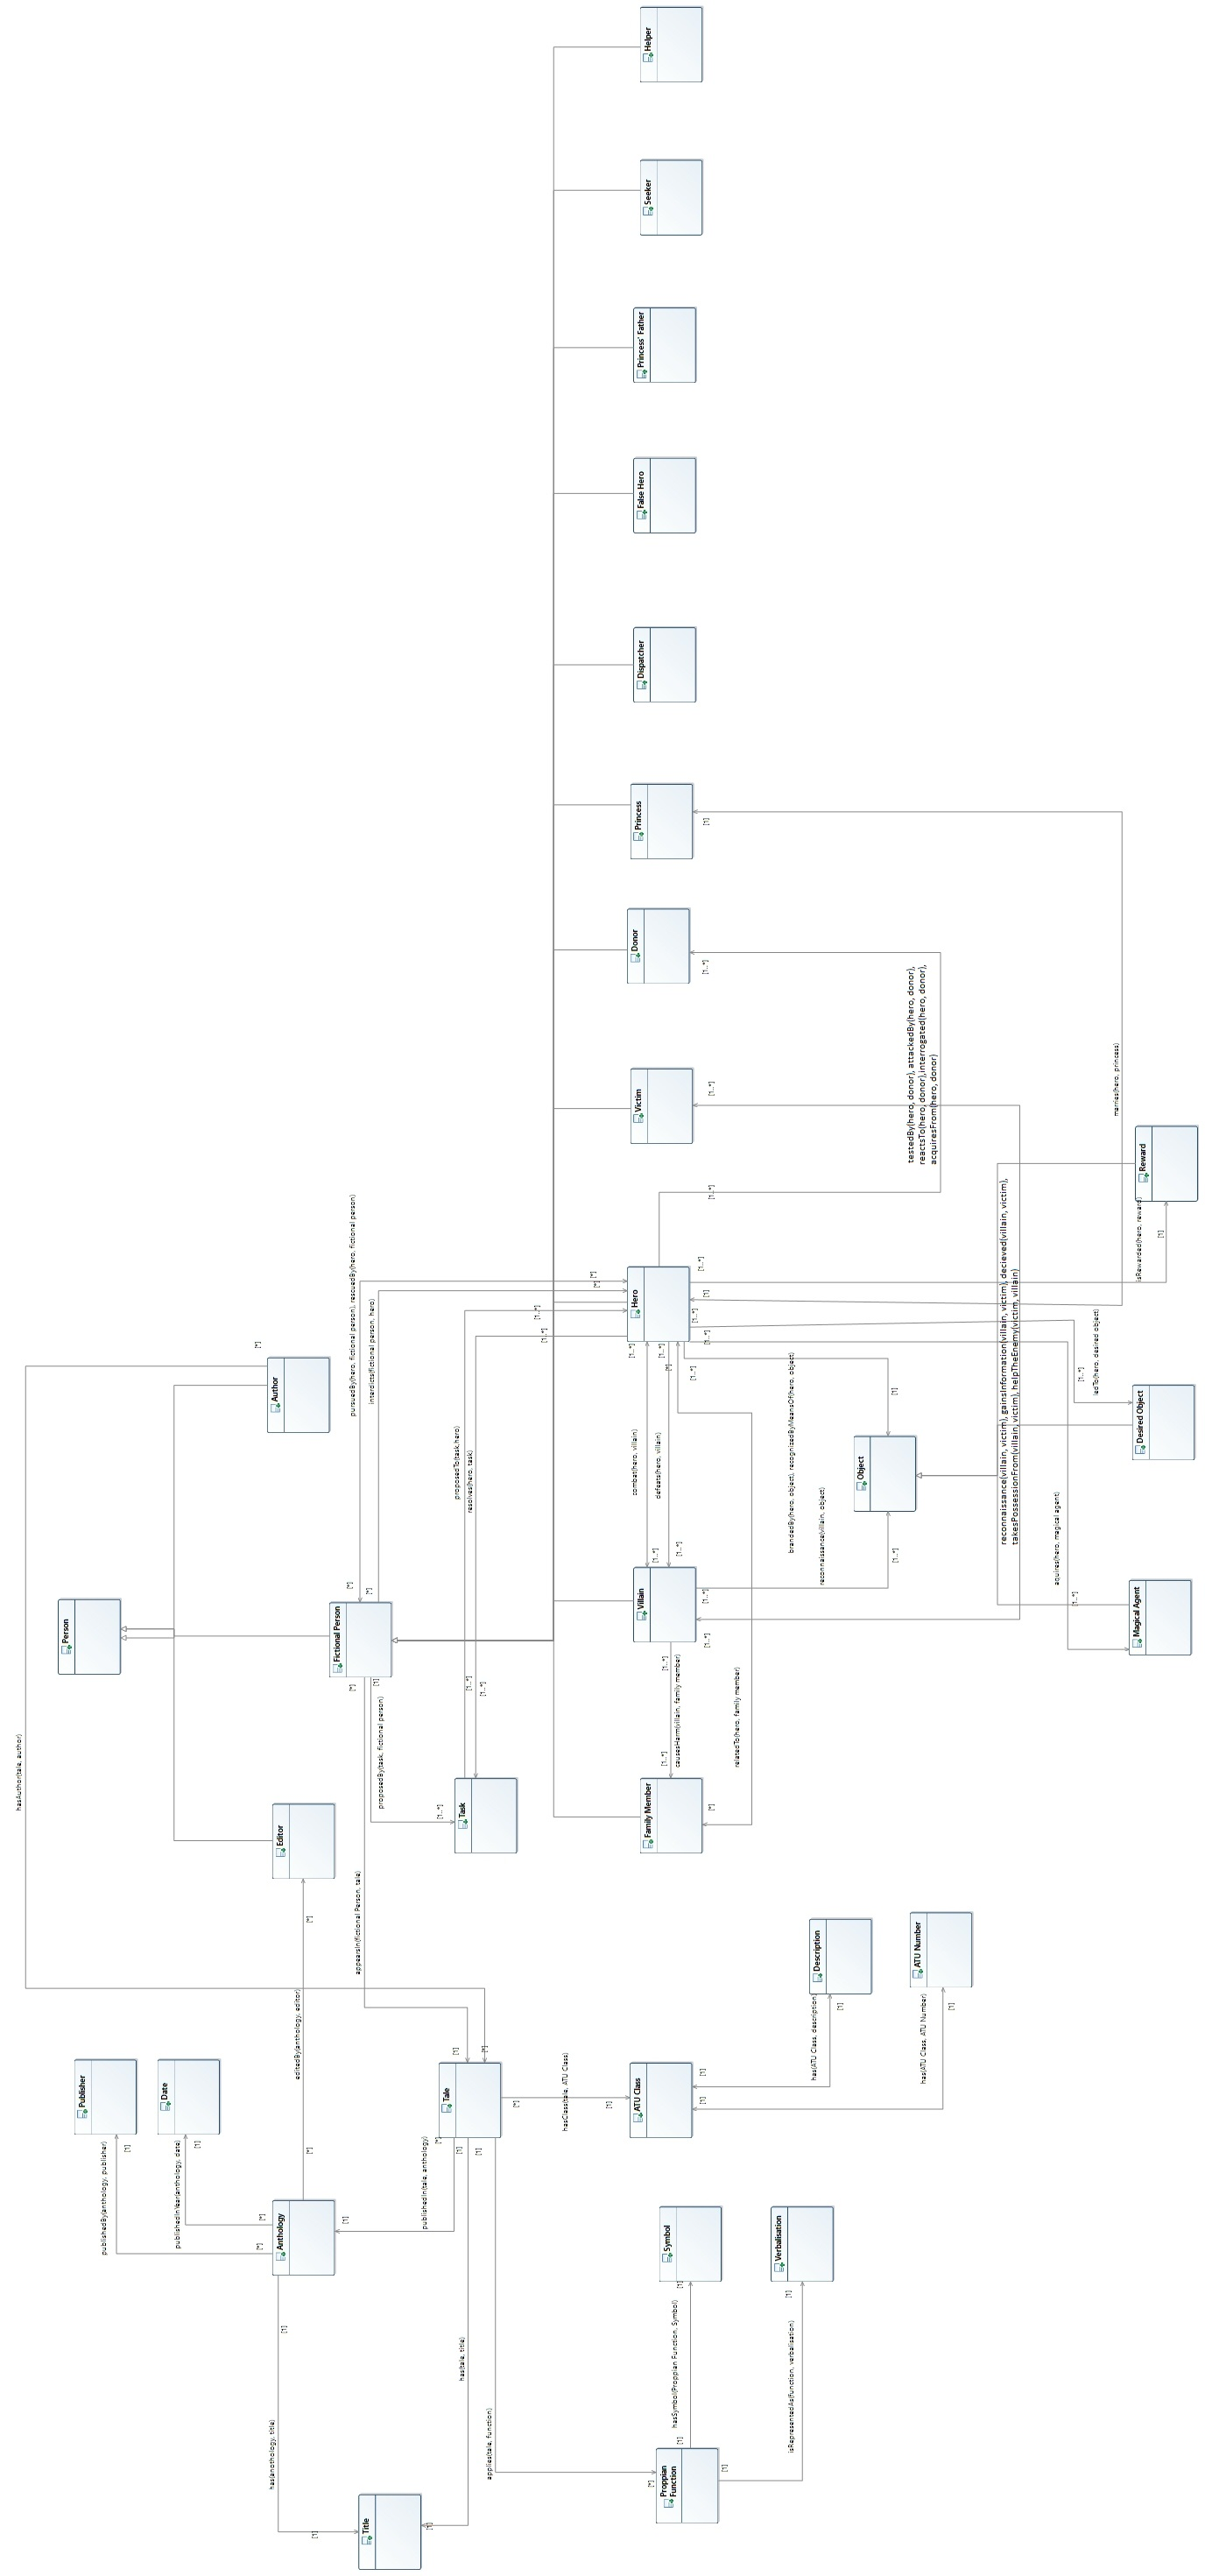
\includegraphics[scale=0.275]{NewModelClassDiagram.jpg}
\end{figure}

\subsection{Description Logic}

\begin{tabular}{c|c|c}
Axioms of Class Hierarchy & Relationship & \\
\hline
FictionalPerson $\subseteq \exists $ isA.Person  & & \\
Hero $\subseteq \exists $ isA.FictionalPerson  & & \\
False Hero $\subseteq \exists $ isA.FictionalPerson  & & \\

Dispatcher $\subseteq \exists $ isA.FictionalPerson  & & \\
Villain $\subseteq \exists $ isA.FictionalPerson  & & \\
Donor $\subseteq \exists $ isA.FictionalPerson  & & \\
Seeker $\subseteq \exists $ isA.FictionalPerson  & & \\
Helper $\subseteq \exists $ isA.FictionalPerson  & & \\
Victim $\subseteq \exists $ isA.FictionalPerson  & & \\
Family Member $\subseteq \exists $ isA.FictionalPerson  & & \\
Princess $\subseteq \exists $ isA.FictionalPerson  & & \\
Princess' Father $\subseteq \exists $ isA.FictionalPerson  & & \\
Editor $\subseteq \exists $ isA.Person  & & \\
Author $\subseteq \exists $ isA.Person  & & \\
Desired Object $\subseteq \exists $ isA.Object  & & \\
Magical Agent $\subseteq \exists $ isA.Person  & & \\



\end{tabular} 


\section{Implementation}
\section{Outview}
\section{Bibliography}
\bibliography{Bibliography} 
\bibliographystyle{ieeetr}

\end{document}
